\documentclass[12pt,border=10pt]{standalone}
\usepackage[dvipsnames,table]{xcolor}
\usepackage{siunitx} % SI-units
\usepackage{pgfplots}
\usepgfplotslibrary{units} % to add units easily to axis
\usepgfplotslibrary{fillbetween} % to fill inbetween curves
\usepgfplotslibrary{colormaps} % to create colormaps
\pgfplotsset{width=12.2cm, height=7cm}
\pgfplotsset{compat=newest} %(making it only compatalbe with
%new releases of pgfplots)
\pgfdeclarehorizontalshading{visiblelight}{50bp}{
color(0.00000000000000bp)=(violet);
color(8.33333333333333bp)=(blue);
color(16.66666666666670bp)=(cyan);
color(25.00000000000000bp)=(green);
color(33.33333333333330bp)=(yellow);
color(41.66666666666670bp)=(orange);
color(50.00000000000000bp)=(red)
}%

\begin{document}
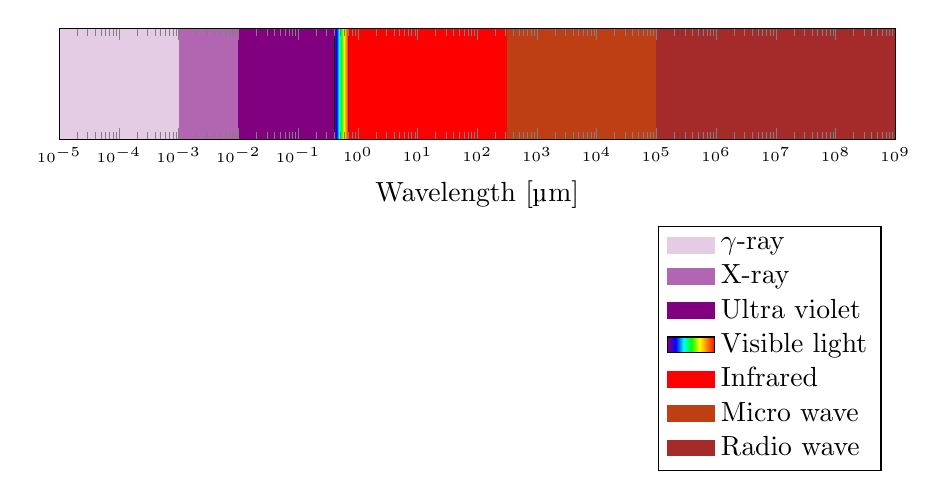
\begin{tikzpicture}[fill between/on layer={axis grid}]
\begin{axis}[
xlabel={Wavelength},
xticklabel style = {font=\tiny,yshift=0.2ex},
xmin=10^-5,
xmax=10^9,
x unit=\si{\micro\meter},
xmode=log,
ymin=0,
ymax=1,
height=3cm,
yticklabels={},
ytick=\empty,
legend cell align=left,
legend style={at={(0.85,-0.77)},anchor=north}
]
\addplot[draw=none, name path=start, forget plot] coordinates{(10^-5,0)(10^-5,1)};
\addplot[draw=none, name path=gamma, forget plot] coordinates{(10^-3,0)(10^-3,1)};
\addplot[draw=none, name path=xrays, forget plot] coordinates{(10^-2,0)(10^-2,1)};
\addplot[draw=none, name path=uv, forget plot] coordinates{(0.4,0)(0.4,1)};
\addplot[draw=none, name path=visible, forget plot] coordinates{(0.7,0)(0.7,1)};
\addplot[draw=none, name path=ir, forget plot] coordinates{(10^2.5,0)(10^2.5,1)};
\addplot[draw=none, name path=microwave, forget plot] coordinates{(10^5,0)(10^5,1)};
\addplot[draw=none, name path=radiowave, forget plot] coordinates{(10^9,0)(10^9,1)};
\addplot[violet!20, area legend] fill between[of=start and gamma];
\addlegendentry{$\gamma$-ray}
\addplot[violet!60, area legend] fill between[of=gamma and xrays];
\addlegendentry{X-ray}
\addplot[violet, area legend] fill between[of=xrays and uv];
\addlegendentry{Ultra violet}
\addplot[shading=visiblelight, area legend] fill between[of=uv and visible];
\addlegendentry{Visible light}
\addplot[red, area legend] fill between[of=visible and ir];
\addlegendentry{Infrared}
\addplot[Bittersweet, area legend] fill between[of=ir and microwave];
\addlegendentry{Micro wave}
\addplot[Brown, area legend] fill between[of=microwave and radiowave];
\addlegendentry{Radio wave}
\end{axis}
\end{tikzpicture}
\end{document}
